\documentclass{article}
\usepackage{lipsum}
% Language setting
% Replace `english' with e.g. `spanish' to change the document language
\usepackage[english]{babel}
% Set page size and margins
% Replace `letterpaper' with `a4paper' for UK/EU standard size
\usepackage[letterpaper,top=2cm,bottom=2cm,left=3cm,right=3cm,marginparwidth=1.75cm]{geometry}

% Useful packages
\usepackage{amsmath}
\usepackage{graphicx}
\usepackage{subcaption}
\usepackage{wrapfig}
\usepackage{pdfpages}
\usepackage{lipsum}
\usepackage{wrapfig}
% \usepackage[colorlinks=true, allcolors=blue]{hyperref}

\usepackage{color}   %May be necessary if you want to color links
\usepackage{hyperref}
\hypersetup{
    colorlinks=true, %set true if you want colored links
    linktoc=all, 
    linkcolor=blue,
}
\usepackage{cleveref}
% More defined colors
\usepackage[dvipsnames]{xcolor}

% Required package
\usepackage{tikz}
\usetikzlibrary{positioning}

\title{The Speed of Thought: Navigate LLM Inference Autoscaling for a Gen AI Application Toward Production}
\author{Geralyn Chong}
\begin{document}
\maketitle
\tableofcontents

\section{Challenges of LLM Inference in Production}
Tokens are units of text that the model processes which generally correspond to 4 characters of text. Time to First Token (TTFT) is the time is takes for the model to generate the first token after recieving a requiest. End-to-end Latency. 

Inference Throughput: concept of a batch where there are multiple sequences that come from different clients. Number of tokens per unit of time. 
\begin{itemize}
    \item Reuqest per second per deployment (RPS)
    \item Tokens per second per deployment (TPS)
    \item Requests per second per GPU
\end{itemize}
Concurrency is NOT throughput: How many tokens are being processed at the same time. \begin{itemize}
    \item Low Concurrency:Results in lower latency due to smaller batch sizes for GPU processing. However, leads to suboptimal throughput and higher cost per token. GPU resources are underutilized
    \item High Concurrency: Improves overall throughput and reduces cost per token. Makes better use of GPU capacity through increased parallel processing. May increase latency due to larger batch sizes
\end{itemize}
Optimizing for Latency or Throughput: 
Online - live generation where you interact with them \textbf{live}. Here latency is really important becuase it matters how quickly they will get hteir repsonse.
Offline - postponed computation refering to the simplest execution of the model where we want to maximize GPU utilization. \\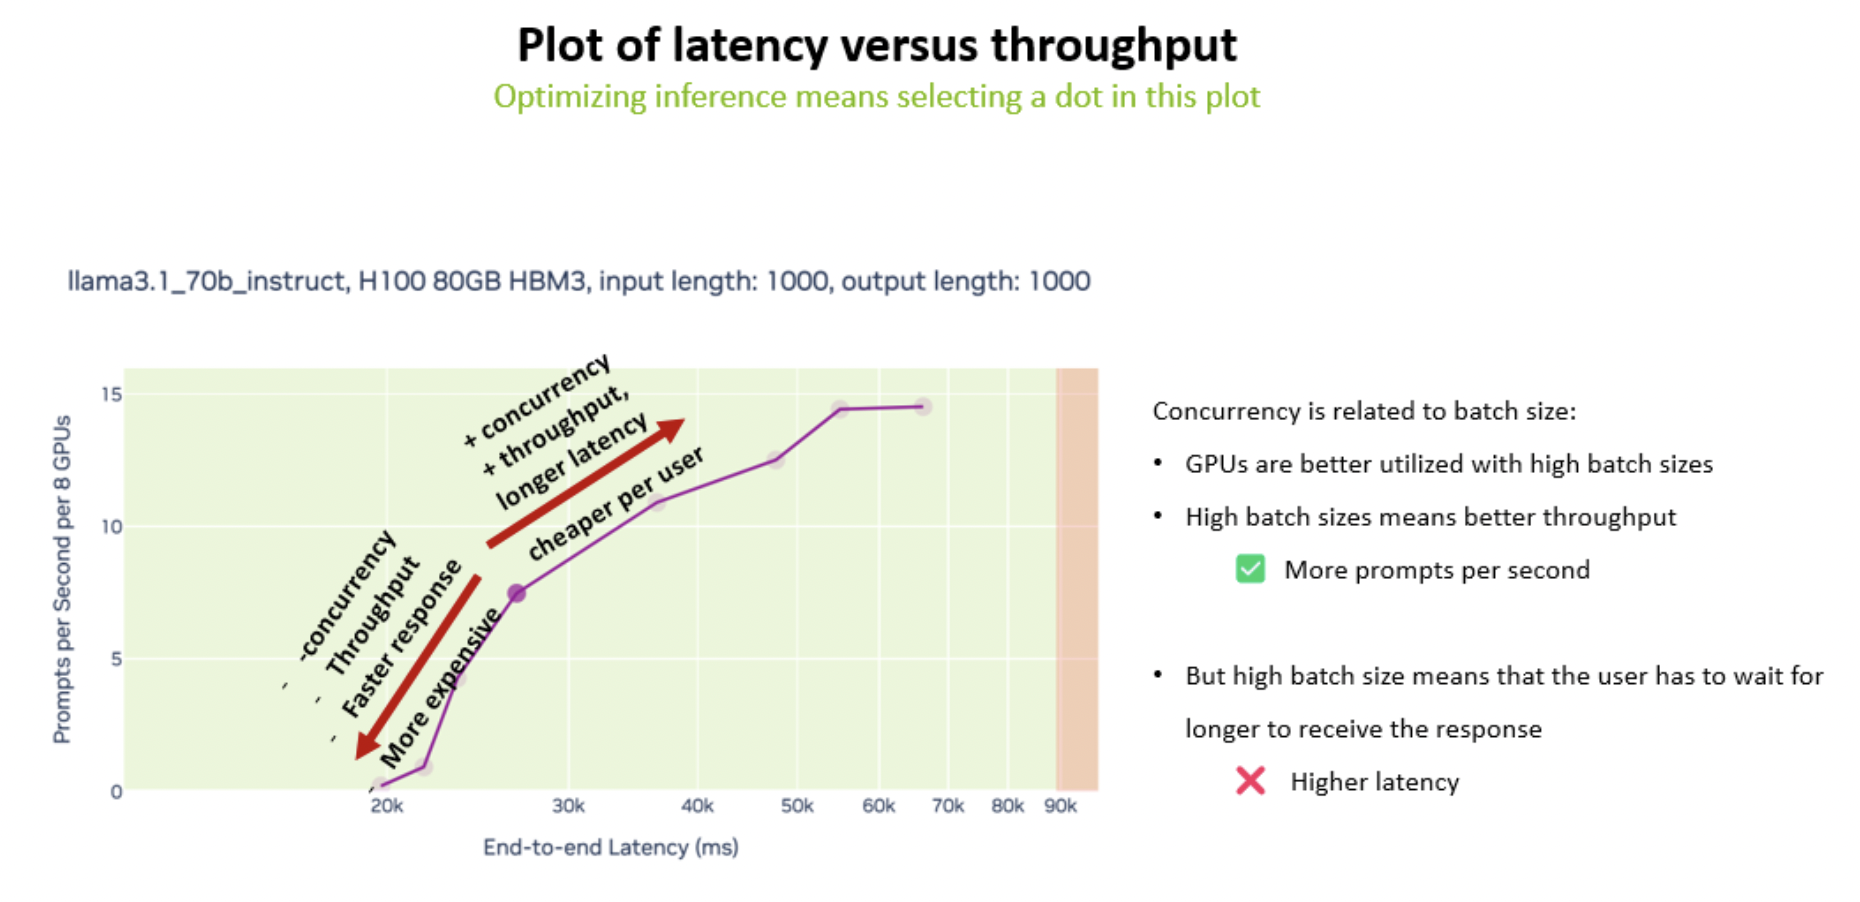
\includegraphics[width=\textwidth]{../images/latencyPlot.png}\\

\subsection{Variables impacting latency vs throughput plot}
\begin{itemize}
    \item Context window (Input length)
    \item Size of the model used
    \item Latency requirement that bounds performance
    \item Size of tokens needed to be produced
\end{itemize}
Autoscaling Example:
What is autoscaling? When there are peaks in the number of requests to our server, how can we manipulate our resources to best support these requests? "How can we keep a similar SLA of latency when the request/s increase?
\begin{enumerate}
    \item Keep same number of 8 GPUs but increase the concurrency: Throughout increases and latency is penalized \\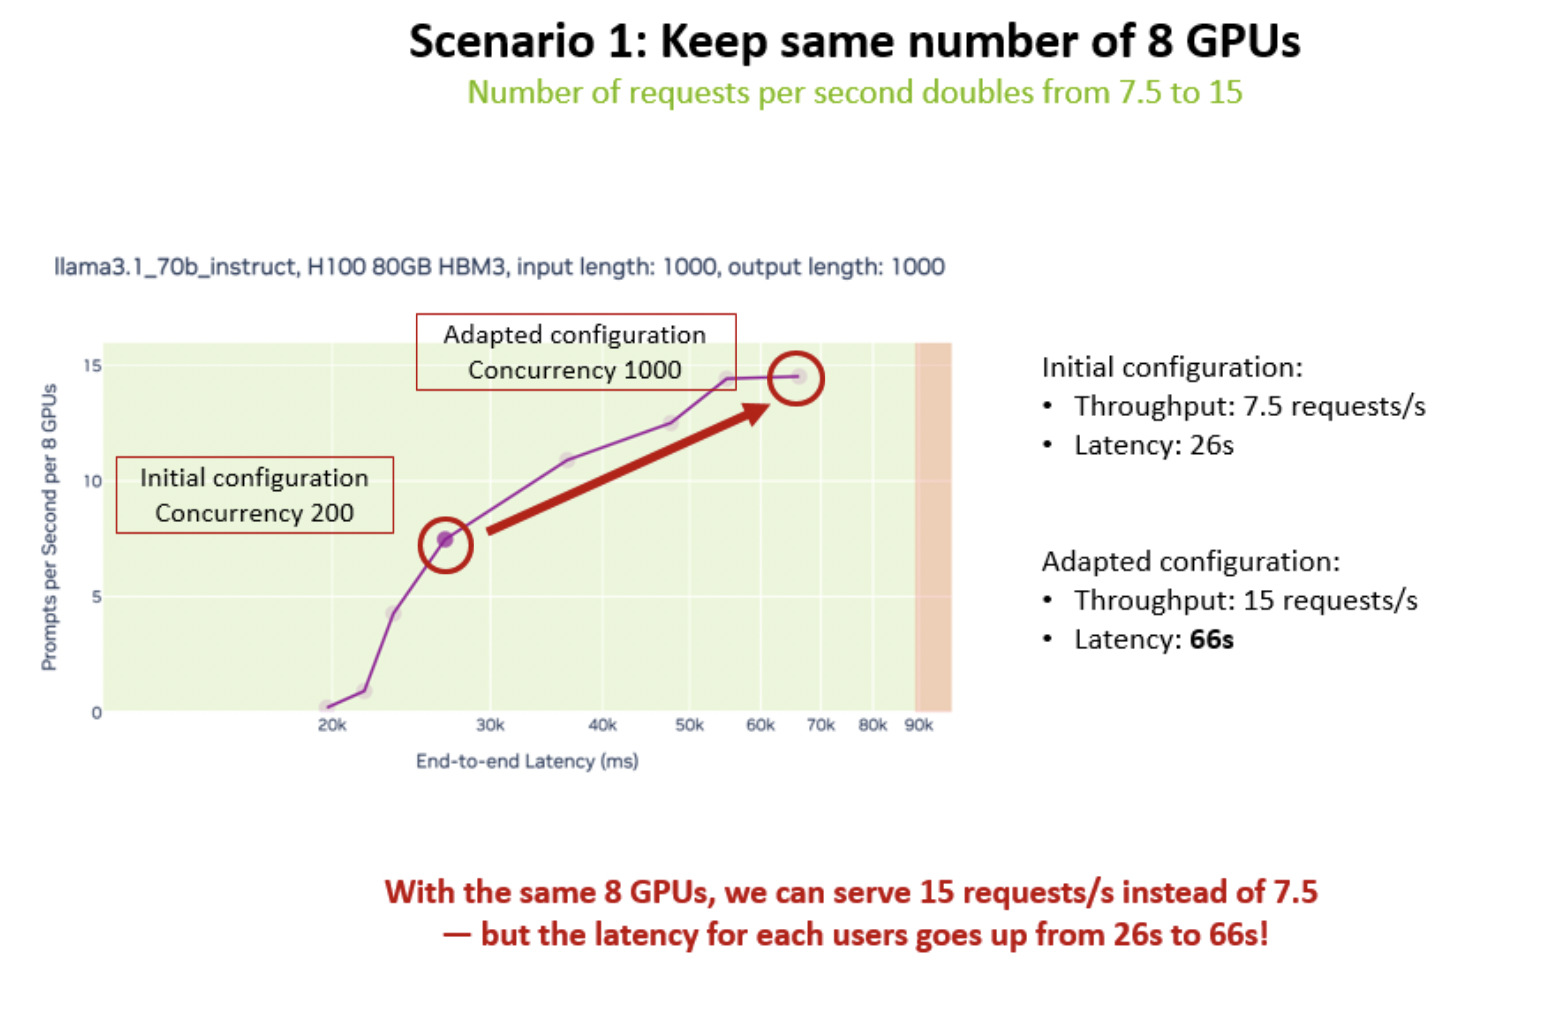
\includegraphics[width=0.8\textwidth]{../images/scenario1.png}
    \item Keep concurrency but autoscale to more GPUs: allow to keep same latency for users but autoscaled pods scale throughput\\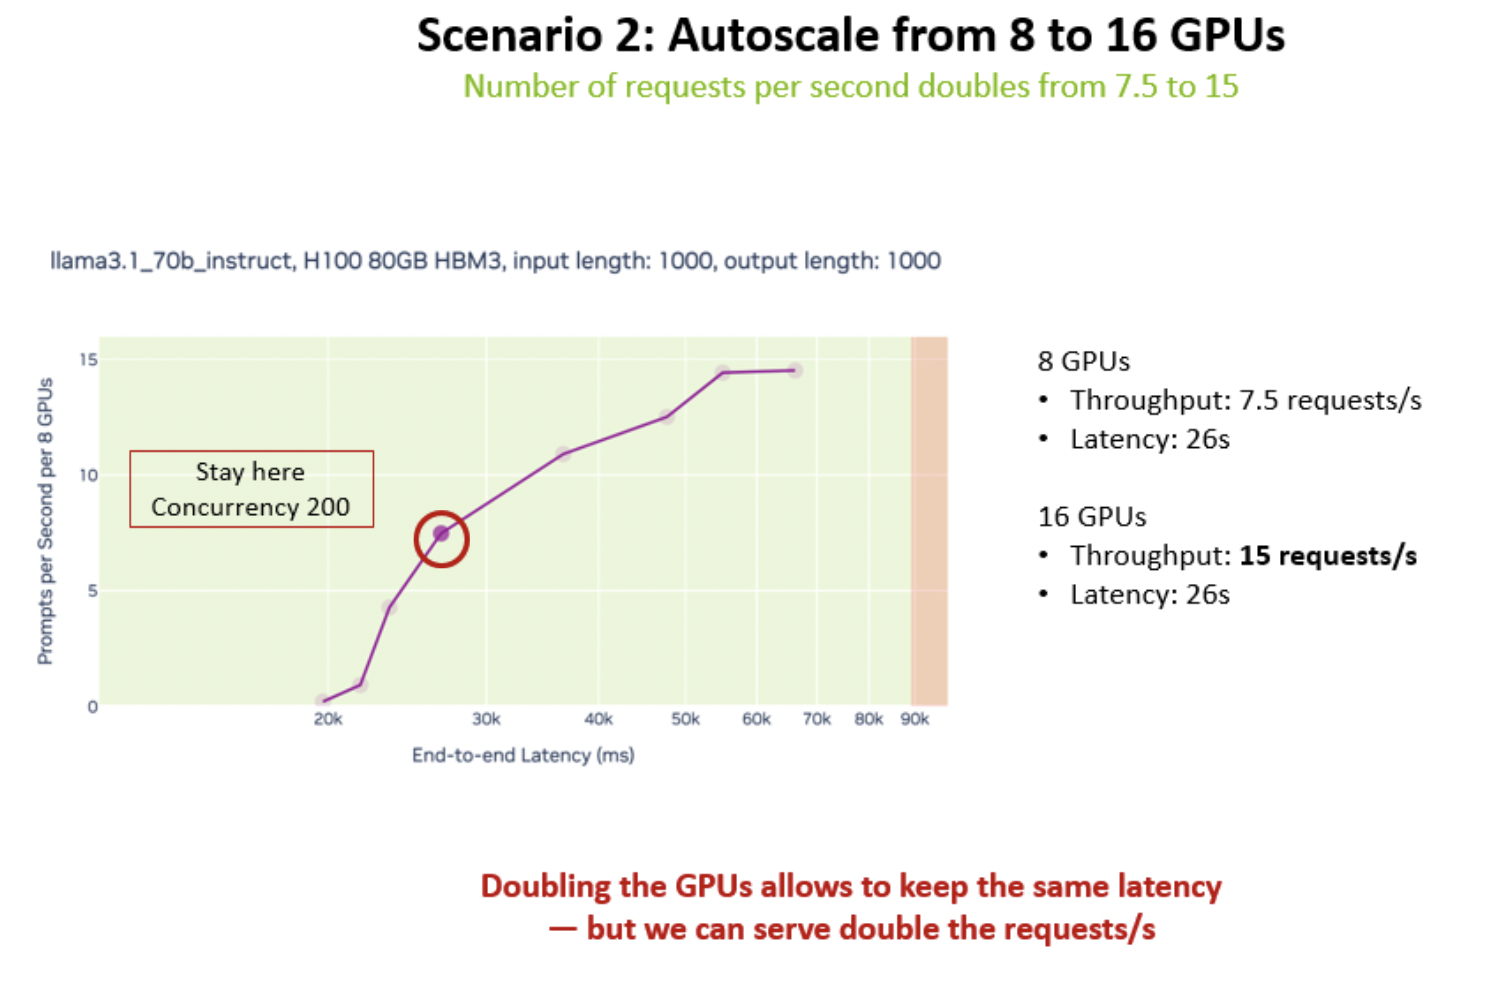
\includegraphics[width=0.8\textwidth]{../images/scenario2.png}
\end{enumerate}

\section{NIMs}
Ease of deployment of LLMs for production and have full control over your own model. Optimized Inference Microservices that have accelerated runtime for gen AI. \begin{itemize}
    \item Portable 
    \item Easy to use
    \item Enterprise Supported
    \item Performance 
\end{itemize}
Applications to many domains.

Internals of NIM: 
\begin{enumerate}
    \item Allows for multiple types of backends
    \item LLM Executor
    \item FastAPI
\end{enumerate}

\section{Lab 1: NIM Operator for K8s}
Lab environment:\\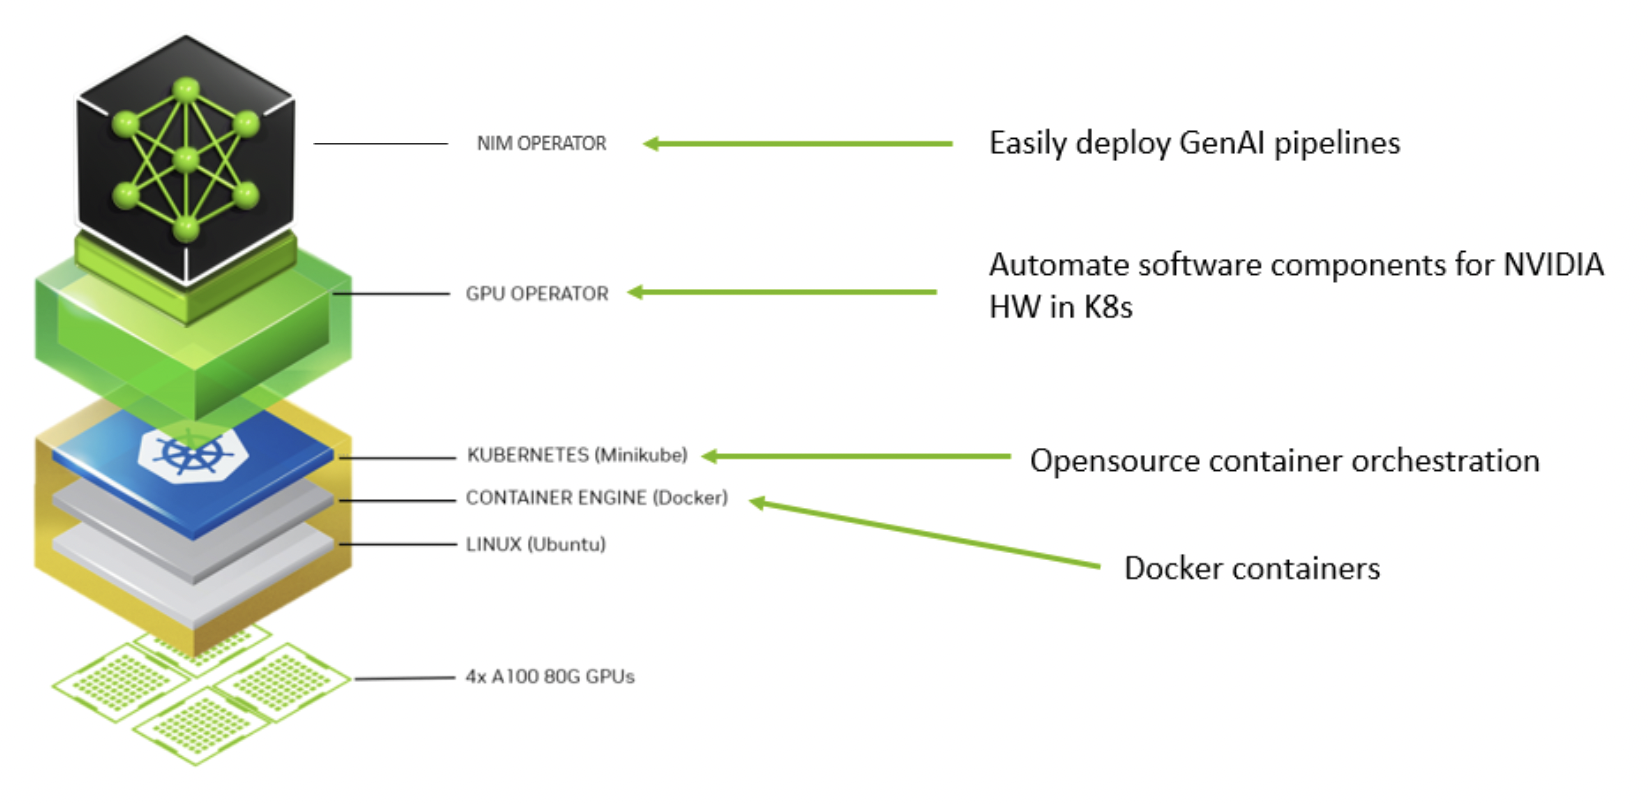
\includegraphics[width=0.9\textwidth]{../images/labenvir.png}
\href{https://docs.nvidia.com/nim-operator/latest/install.html}{text}

The NIM operator introduces two essential custom resources that work together to deploy AI models: \begin{enumerate}
    \item NIM Cache: Downloads models from NVIDIA NGC - GPU Cloud and storing them persistently on network storage for future use
    \item NIMService: his resource takes a model from an existing NIMCache and deploys it as a microservice, making it available for inference requests.
    \textit{What are inference requests?} Running live data that the model has not seen before in order to produce predictions or complete tasks. 
\end{enumerate}
\section{Benchmarking NIM}
Simulate a certain load of client requests and measure from the client-side the time to get response to calculate latency and trhoughput. Focusing on GenAI-Perf to compute metrics of latency, throughput, and concurrency with ease. Locust is also another tool for measuring these stats. 

This tool allows us to compare these measurement of statistics across different LLM providers. \href{https://docs.nvidia.com/nim/benchmarking/llm/latest/index.html}{Docs}. \\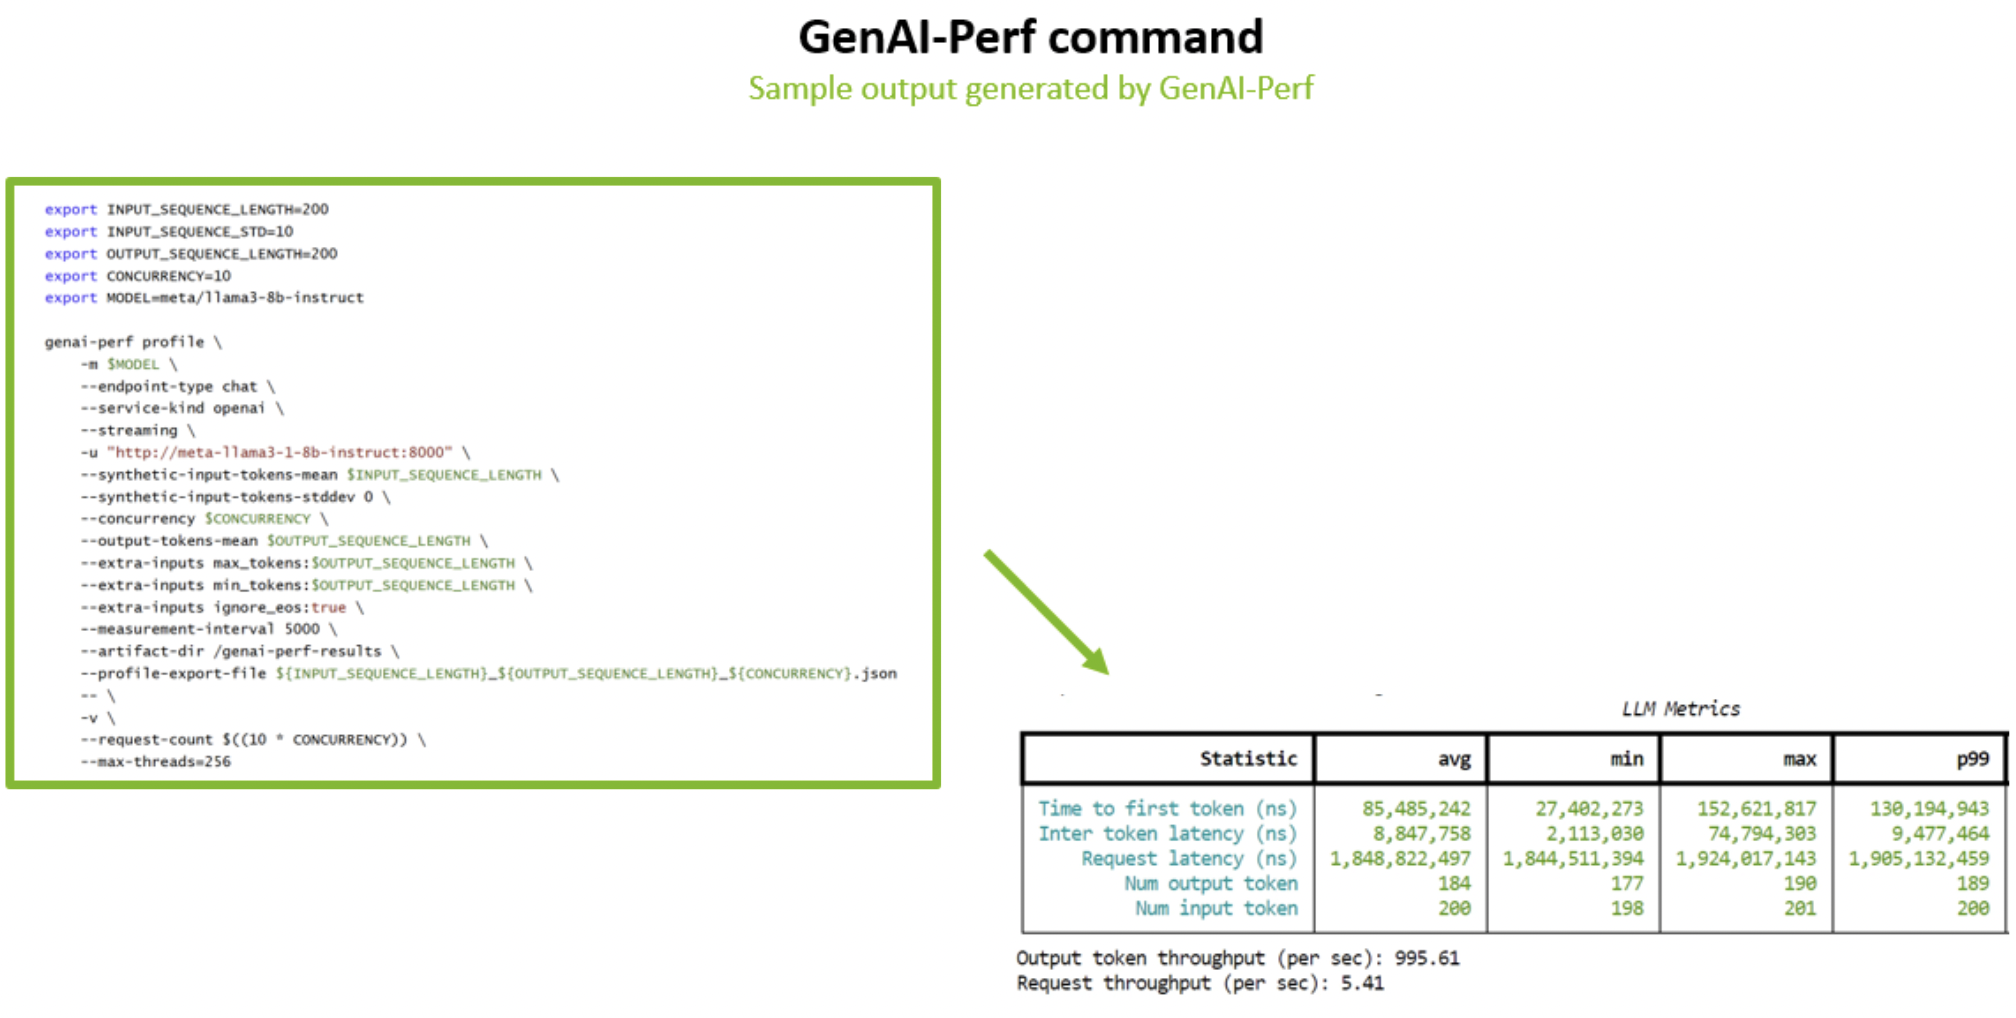
\includegraphics[width=0.9\textwidth]{../images/exampleGenAIperfOutput.png}\\


\section{Observability}
Promethus is an open-source tool that allows us to monitor and alert on the resources used of our system. 
Gauge Metrics represent the current value of the fraction of the GPU memory devoted for the KV-cahce that is being utilized by our model.
Counter Metrics cannot decrease. 
Histogram Metrics divide data into "buckets" that count observation falling within specific ranges. Each bucket has le that defines its upper bound. 
\begin{itemize}
    \item le: less or equal to the value
    \item le='+inf': shows the total number of requests because all latency will be less than $\infty$. 
\end{itemize}
Monitoring the NIM containers: \\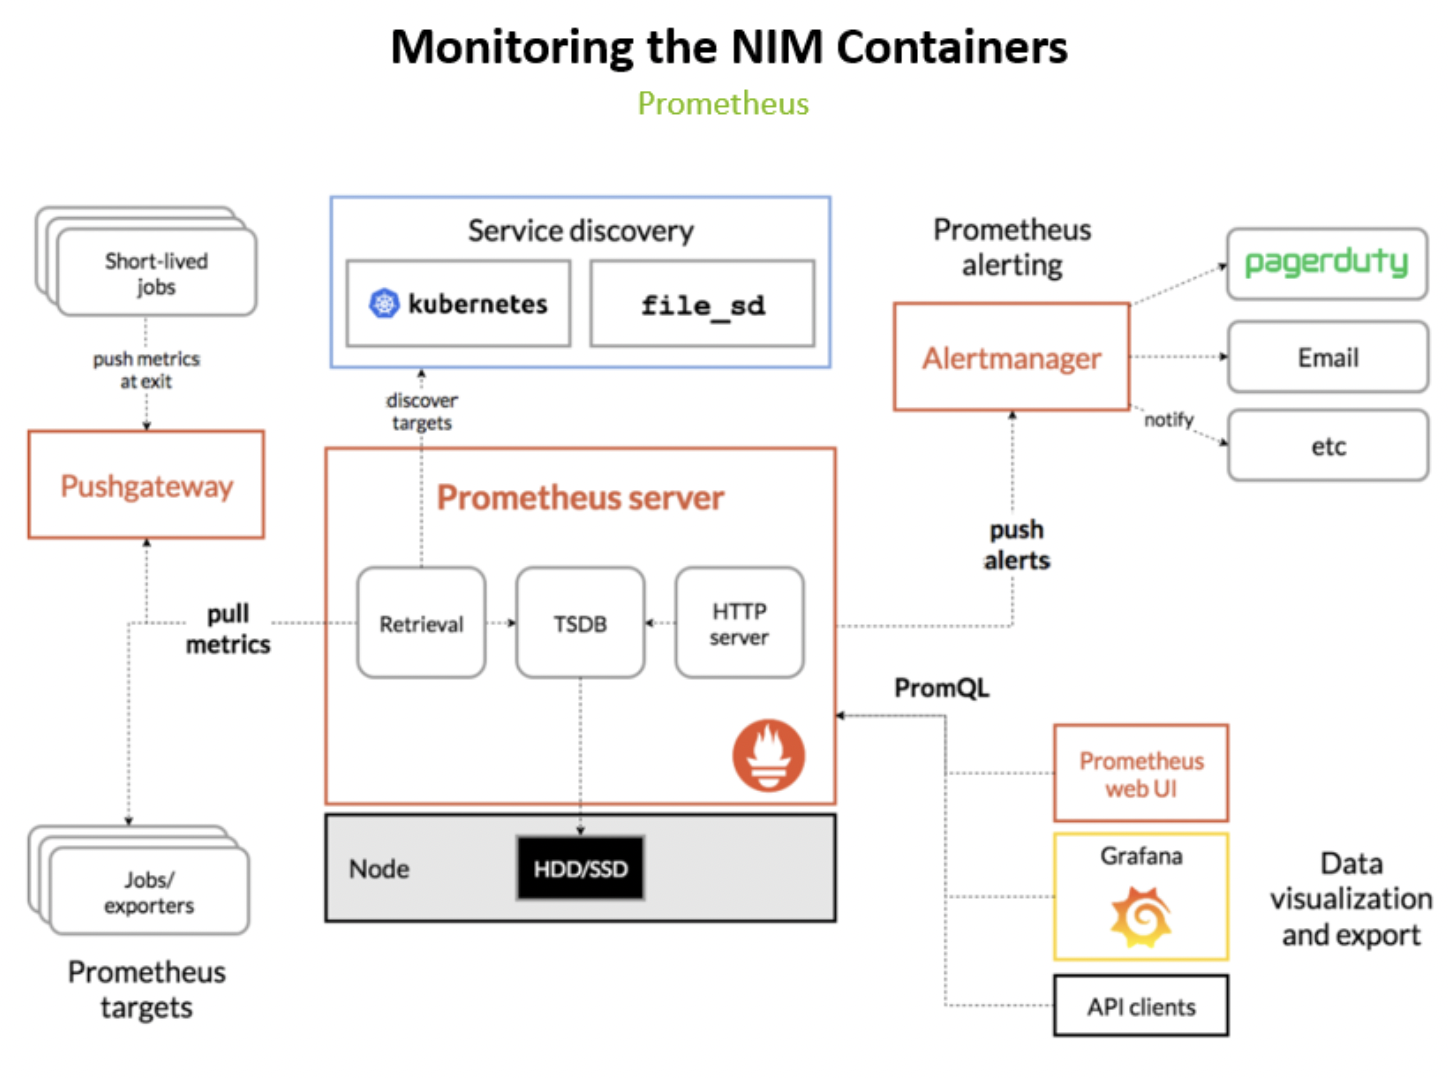
\includegraphics[width=0.9\textwidth]{../images/archPromethus.png}\\
Obtaining GPU Metrics via DCGM Exporter can be done as well. 

NVIDIA NIM provides monitoring of NIM Service level metrics and NIM Operator metrics. Service level metrics are taken from service pods focusing of the model's performance and resource utilization. Operator metrics are collected from Operator pods and track the number of instances in various states. The following code snippets are taken from the lab: 
\begin{itemize}
    \item Grabbing the Gauge metrics ($1 = 100\% of GPU$ used)
    \begin{verbatim}
!curl -Ns -X "GET" "{NIM_ENDPOINT}/v1/metrics" | grep "gpu_cache_usage_perc"
    \end{verbatim}
    \begin{enumerate}
        \item A help message: explains what the message means
        \item Type declaration of the metric: \verb|gauge|
        \item The actual measurement data
    \end{enumerate}
    When multiple models are loaded each model gets its own metric with unique label sets. 
\end{itemize}
\section{Autoscaling with custom metrics}
Autoscaling based on the user workload. \\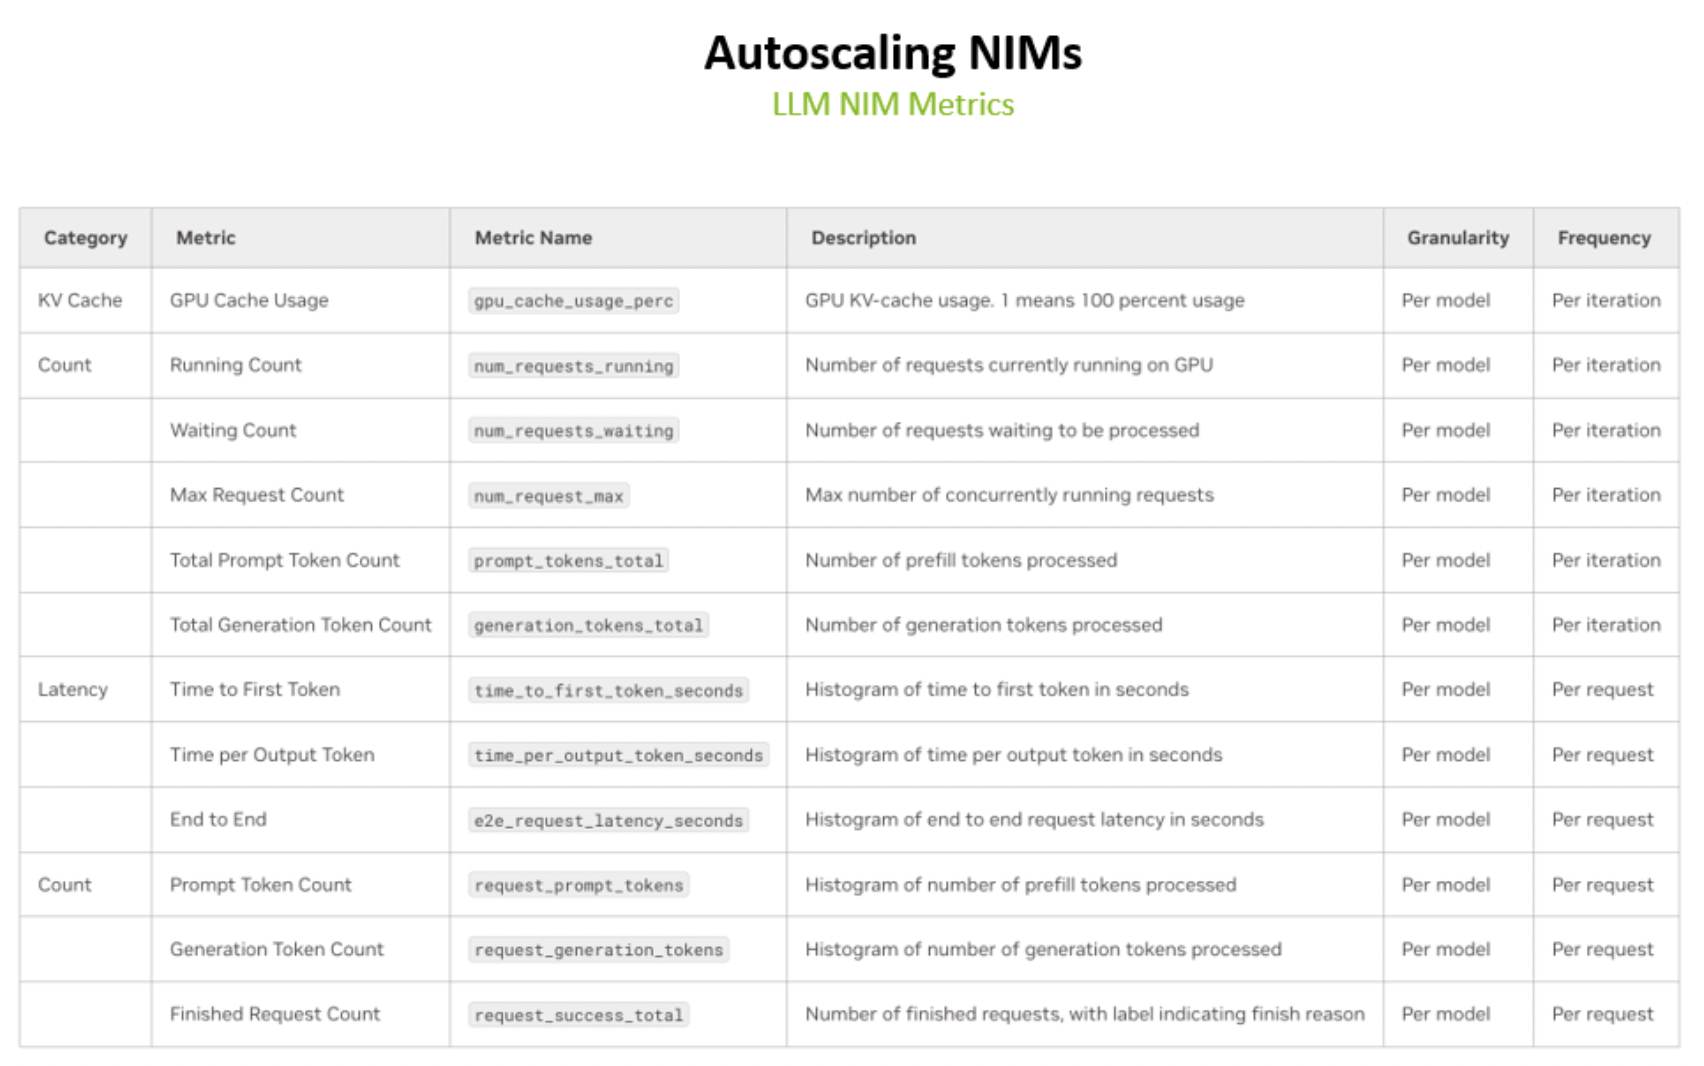
\includegraphics[width=\textwidth]{../images/typesOfmetrics.png}\\
Types of Autoscaling in Kubernetes: 
Focusing on HPA (Horizontal Pod Autoscaler) which increased replica count based on provided metrics. 
Scaling specification in NIMService: need to specifyy the custom metric for GPU usage as well as the average value across the pods used. 

Get HPA controller which is responsible for Autoscaler in each container. Here we then use the generating load test using Locust. Using a constant throughput function, we ensure that users send a reuqest every $x$ seconds. In locust, we ensure that each user generates as many request as possible but to some configured extent. RPS = $\text{num of users} * 0.01$ = Spawn rate.
\begin{wrapfigure}{l}{0.4\textwidth}
    \begin{center}
        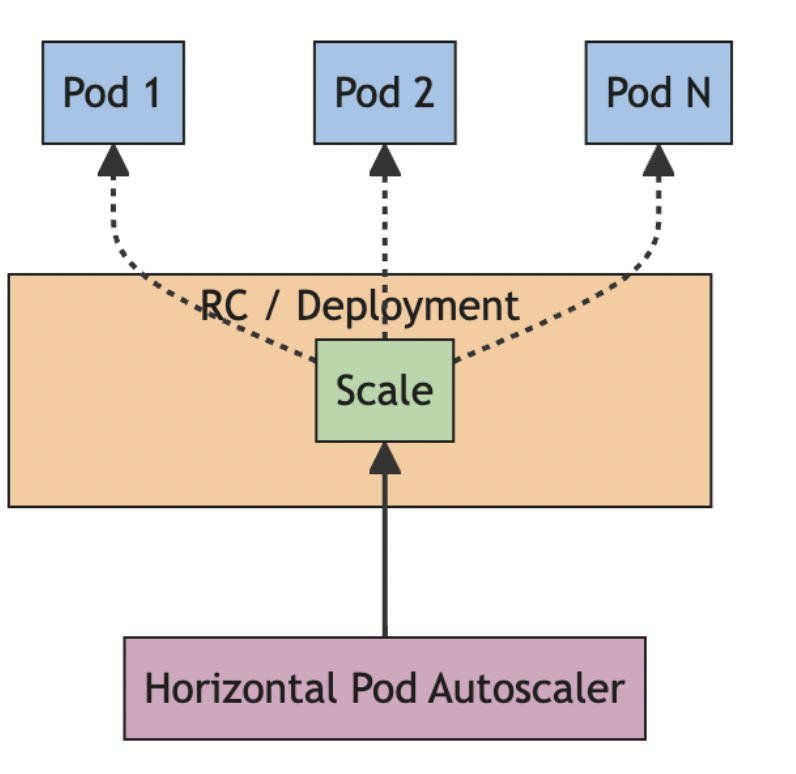
\includegraphics[width=0.3\textwidth]{../images/hpaStructure.png}
    \end{center}
  \end{wrapfigure} There are other methods of autoscaling as well such as the Vertical Pod Autoscaler (VPA) adjusting the resource requests and limits of individual pods to match actual usage. VPA is beneficial for applications with predictable and stable workloads, where resource requirements may vary over time. Cluster Autoscalers automatically adjust the size of the node pool in a cluster. \\\begin{wrapfigure}{r}{0.4\textwidth}
    \begin{center}
        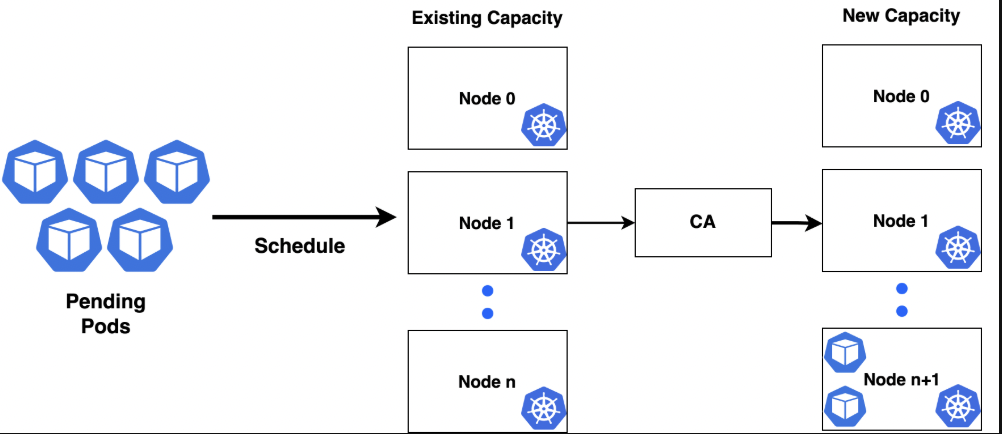
\includegraphics[width=0.3\textwidth]{../images/cpa.png}
    \end{center}
  \end{wrapfigure} For example, when there are insufficient nodes, CA provides more nodes and underutilized nodes are removed. By working with cloud provider APIs, it is able to scale the infrastructure. 
\end{document}